\documentclass[MASTER.tex]{subfiles}
\begin{document}
	%==============================================%
\begin{frame}
\begin{figure}
\centering
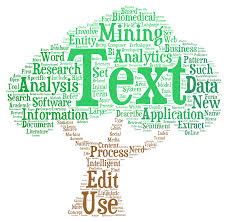
\includegraphics[width=0.75\linewidth]{testmining}

\end{figure}
	
	
\end{frame}
%==============================================%	
\begin{frame}
	\frametitle{gensim}
	\begin{figure}
		\centering
		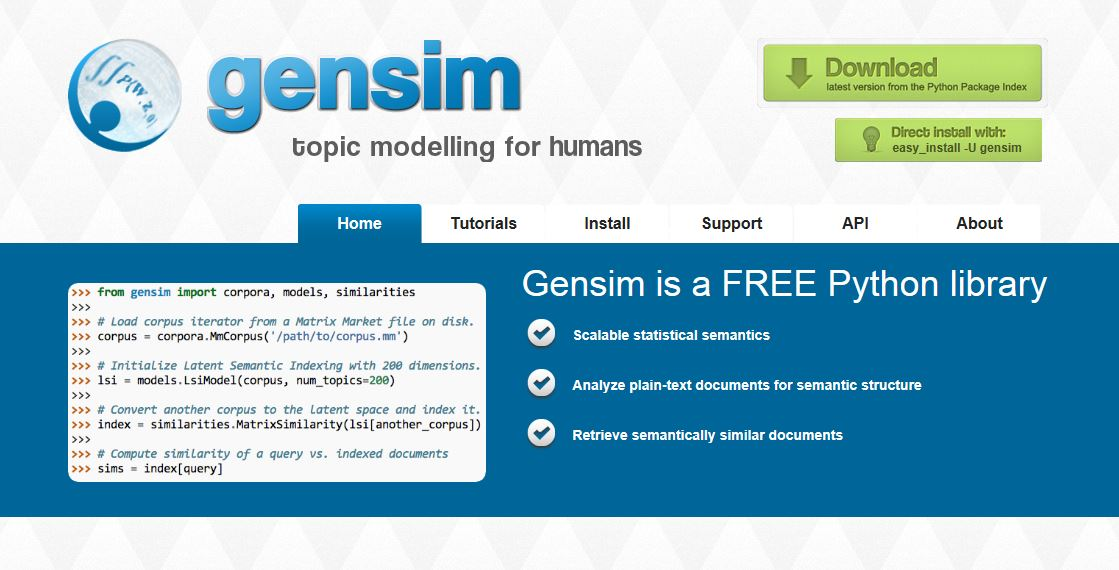
\includegraphics[width=1.05\linewidth]{gensim}

	\end{figure}
\end{frame}
%===========================================%
\begin{frame}
	\frametitle{gensim}
\begin{figure}
	\centering
	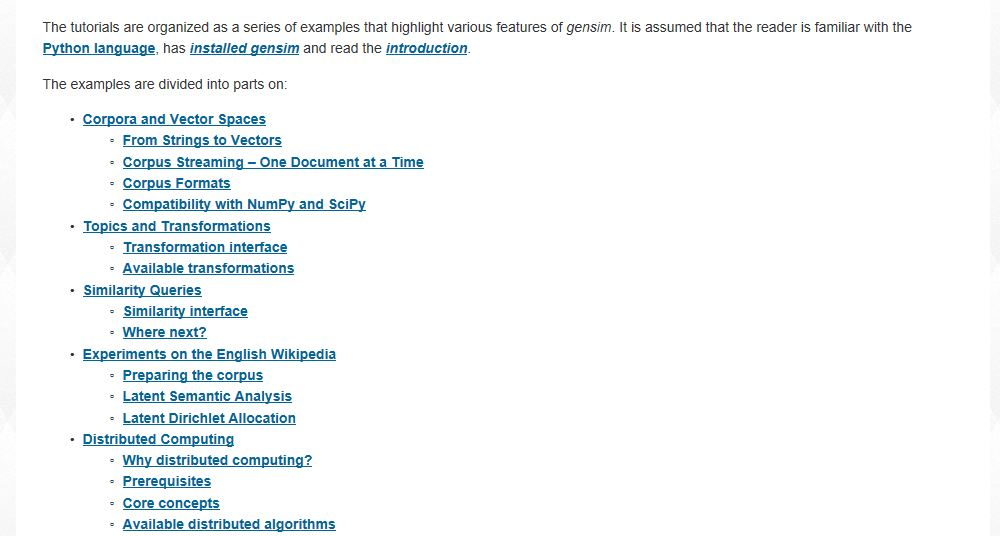
\includegraphics[width=1.05\linewidth]{gensimtutorials}

\end{figure}
\end{frame}
%===================================================%
\begin{frame}
	\frametitle{Beautiful Soup}
	\begin{figure}
\centering
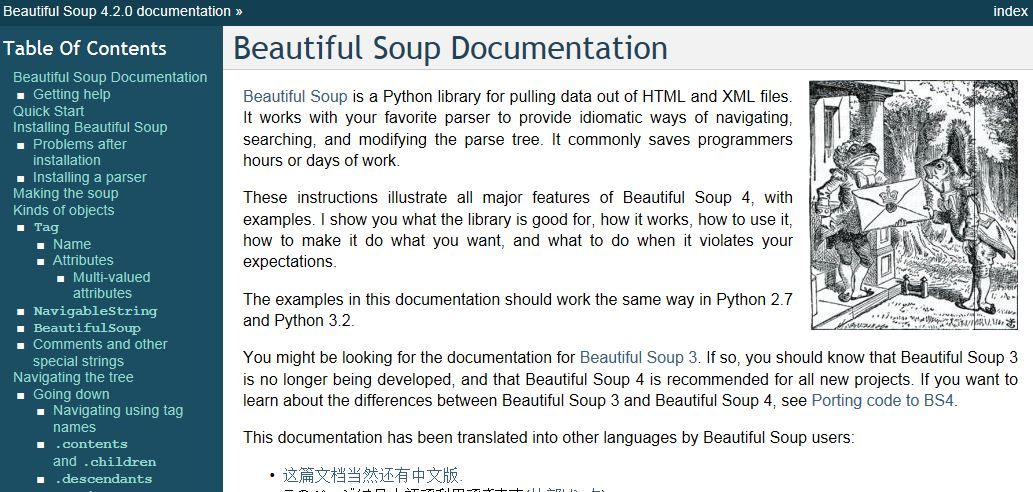
\includegraphics[width=1.05\linewidth]{beautifulsoup}

\end{figure}

\end{frame}
%====================================================%
\begin{frame}
\frametitle{Beautiful Soup}
\textbf{Beautiful Soup}\Large
\large
\begin{itemize}
\item Beautiful Soup is a Python library for pulling data out of HTML and XML files. 
\item It works with your favorite parser to provide idiomatic ways of navigating, searching, and modifying the parse tree. 
\item It commonly saves programmers hours or days of work.
\end{itemize}
\end{frame}
%====================================================%
\end{document}